\section{Bayesian Trust}
\begin{frame}
\frametitle{Bayesian Trust Framework}
%\framesubtitle{Introduction}

Implemented B-Trust~\citep*{btrust}, because some if it's desirable properties
include:
\begin{itemize}
  \item Linearly scalability wrt. \# of Peers;
  \item Subjectiveness;
  \item Context-dependence; and
  \item Dynamism.
\end{itemize}

\end{frame}


\subsection{Theory}
\begin{frame}
\frametitle{Bayesian Trust Framework}
\framesubtitle{Theory I}

Adapted B-Trust~\citep*{btrust}.

\begin{figure}
\begin{equation}
\mu_{\{d,r\}} = \sum_{i=0}^{n-1}{i*{\{d,r\}}_i}
\end{equation}
\caption{Mean}
\end{figure}

\end{frame}


\begin{frame}
\frametitle{Bayesian Trust Framework}
\framesubtitle{Theory II}

\begin{figure}
\begin{equation}
\sigma^2_{\{d,r\}} = \sum_{i=0}^{n-1}{i^2*{\{d,r\}}_i} - \mu^2_{\{d,r\}}
\end{equation}
\caption{Variance}
\end{figure}

\begin{figure}
\begin{equation}
c = 1 - \frac{\sigma^2_{\{d,r\}}}{\sigma^2_U}
\end{equation}
\caption{Confidence}
\end{figure}

\end{frame}


\subsection{Implementation}
\begin{frame}
\frametitle{Bayesian Trust Framework}
\framesubtitle{Implementation I}

\begin{figure}[h!]
  \centering  
  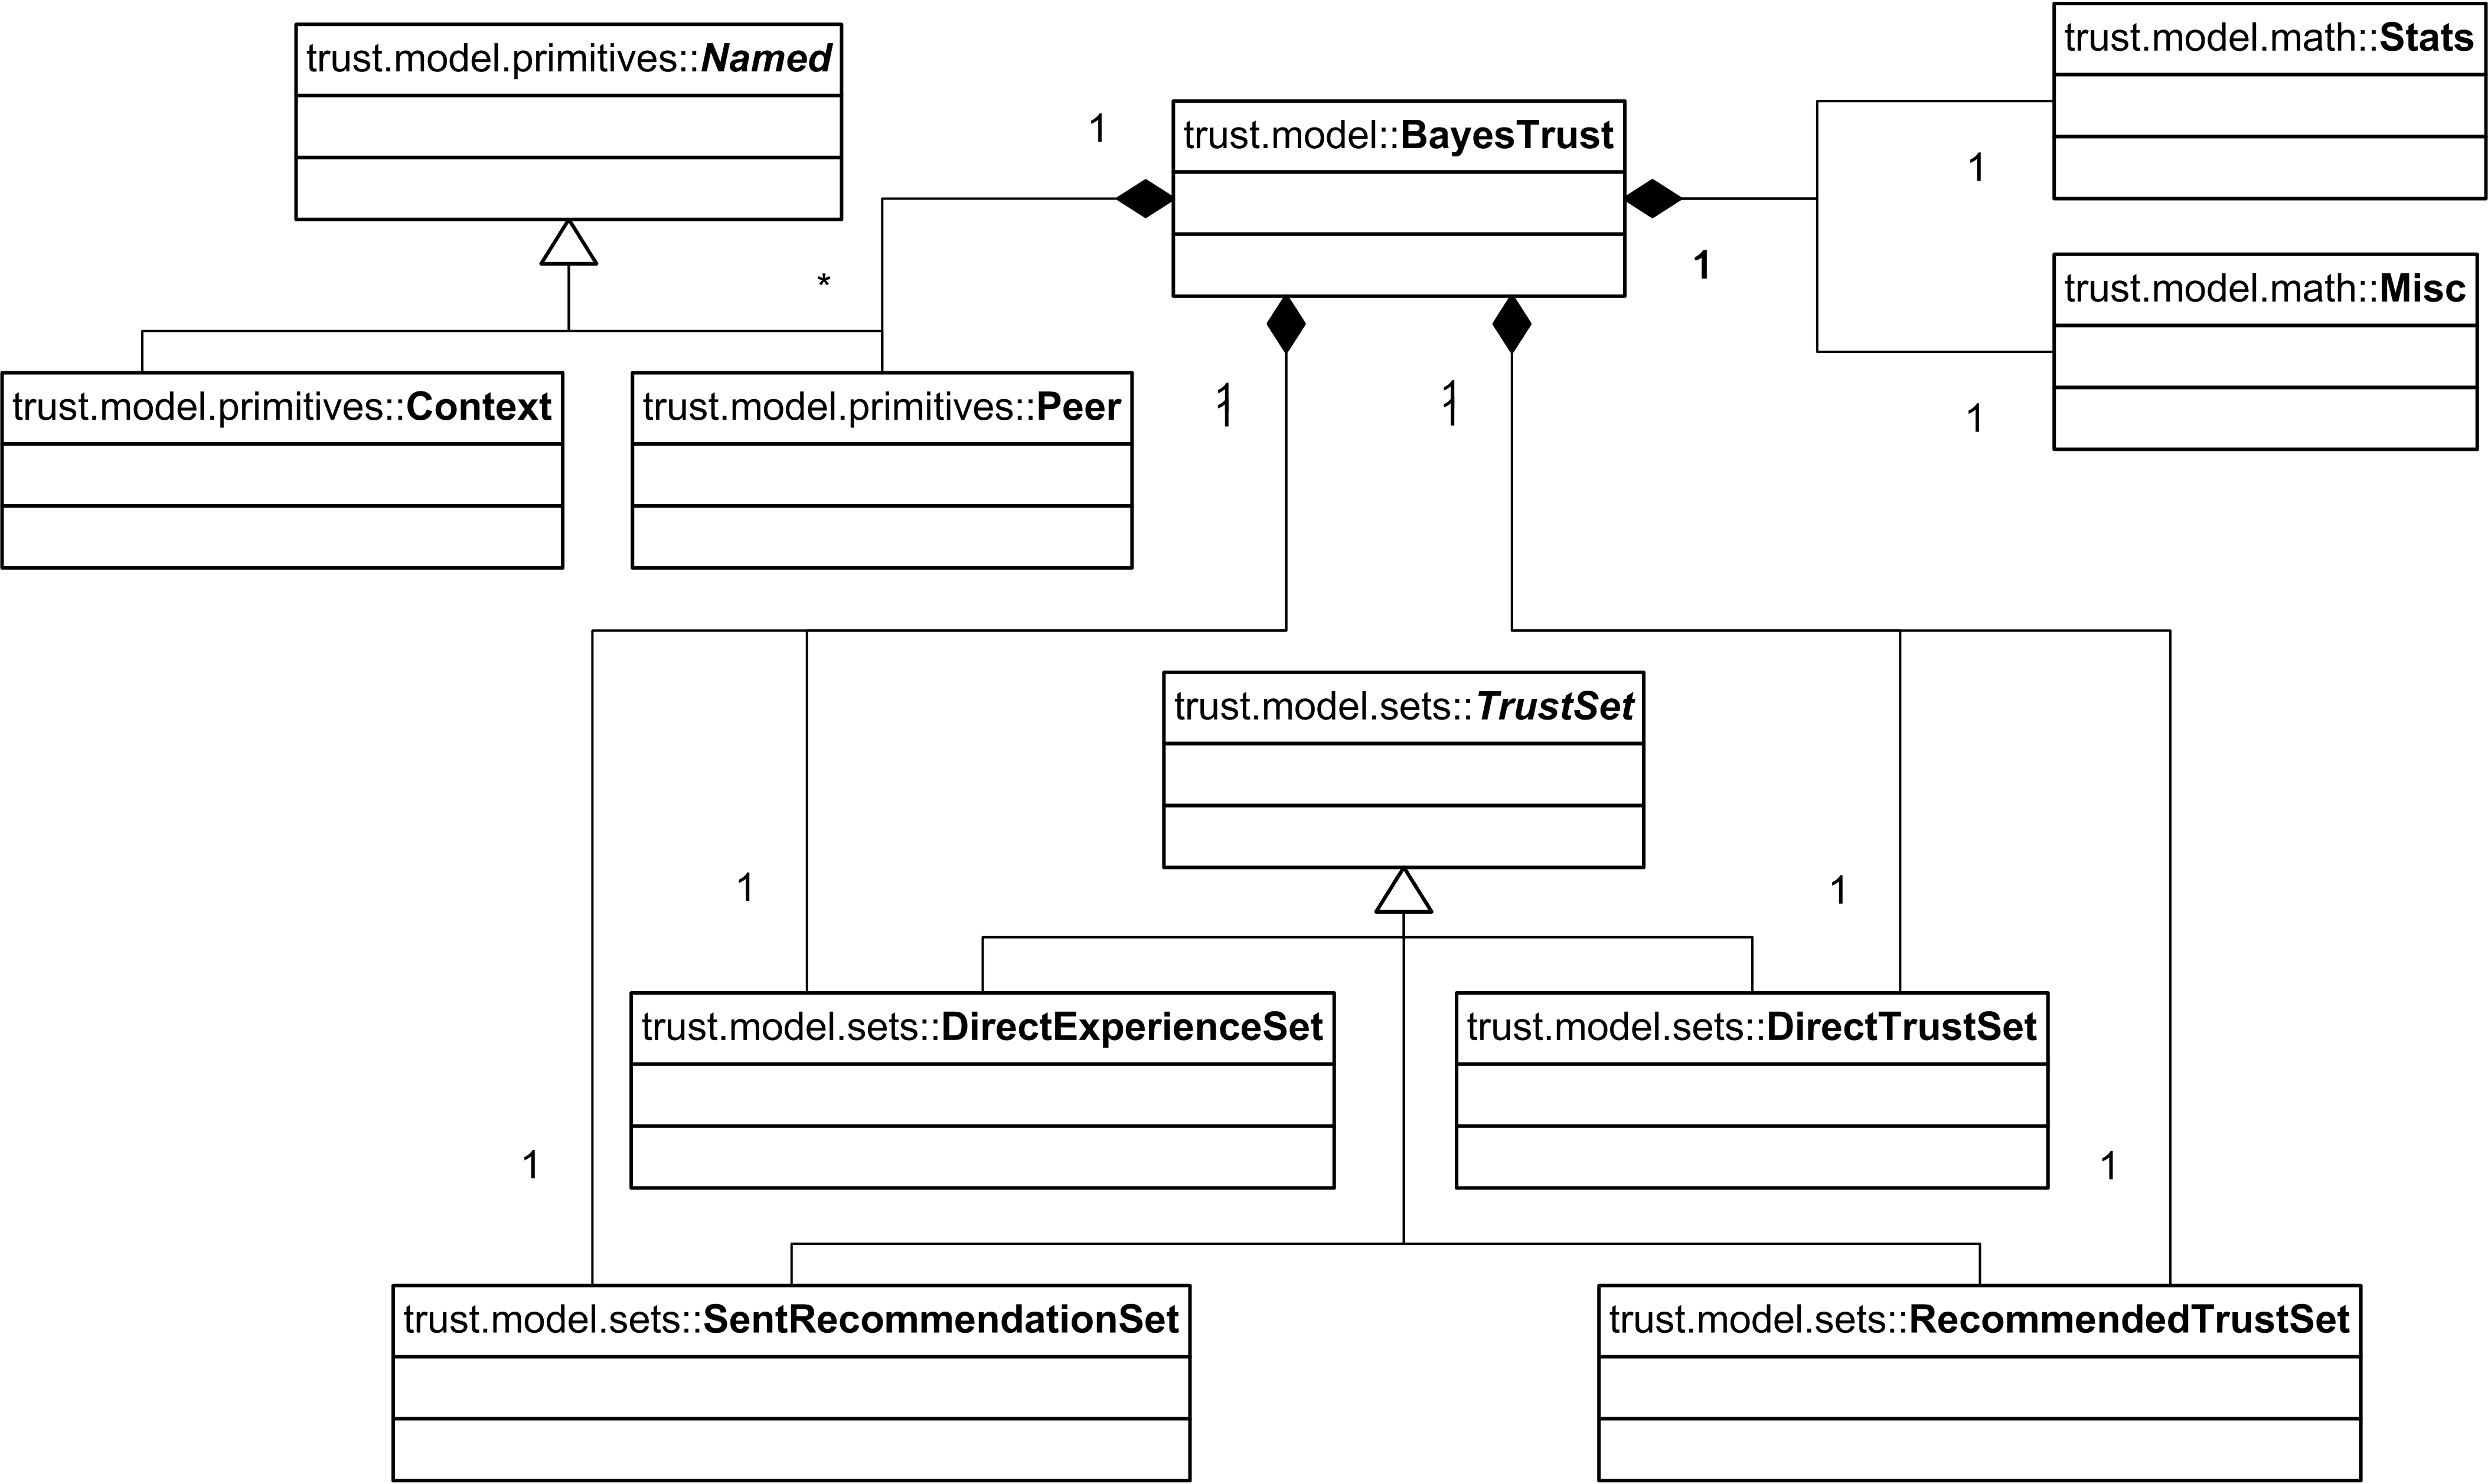
\includegraphics[width=1\textwidth]{../report/images/bayestrust}
\end{figure}

\end{frame}


\begin{frame}
\frametitle{Bayesian Trust Framework}
\framesubtitle{Implementation II}

\begin{figure}[h!]
  \centering  
  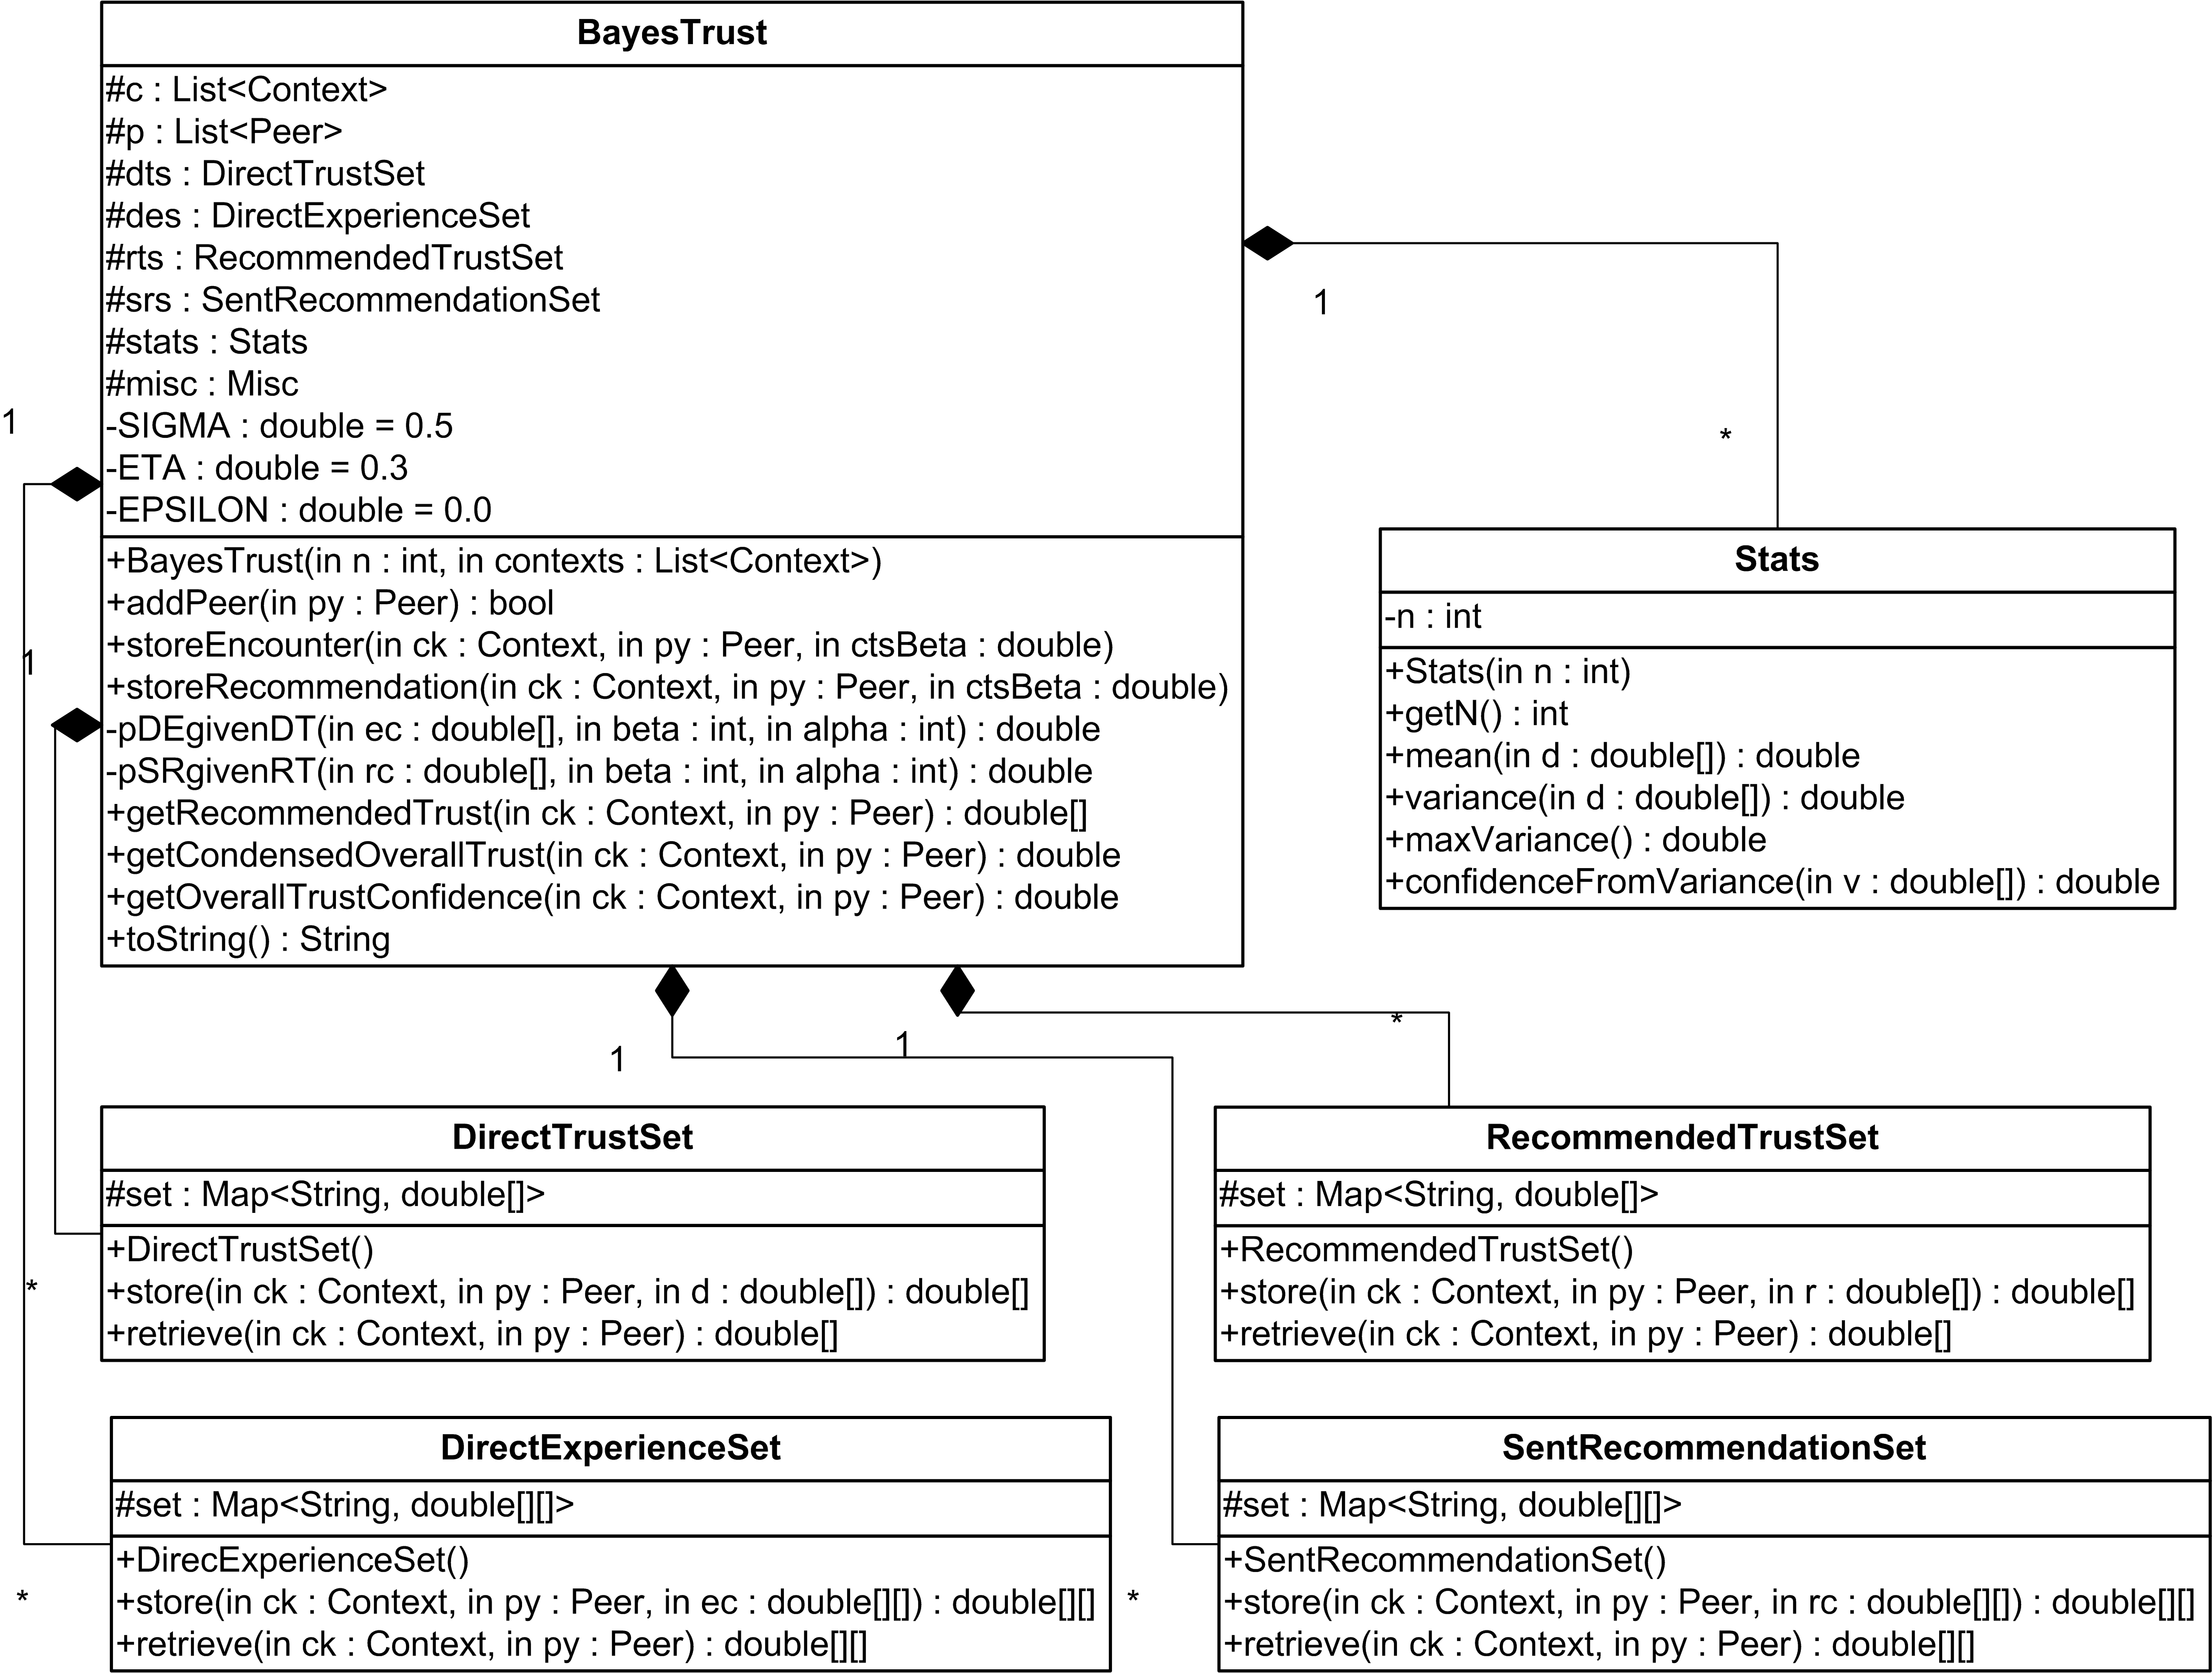
\includegraphics[width=0.9\textwidth]{../report/images/bayestrustdetail}
\end{figure}

\end{frame}